\hypertarget{serial_8cpp}{}\section{src/serial.cpp File Reference}
\label{serial_8cpp}\index{src/serial.\+cpp@{src/serial.\+cpp}}


Implements serial interface to a TS sensor using native Unix command structures.  


{\ttfamily \#include \char`\"{}toposens\+\_\+driver/serial.\+h\char`\"{}}\newline
{\ttfamily \#include $<$fcntl.\+h$>$}\newline
{\ttfamily \#include $<$ros/console.\+h$>$}\newline
{\ttfamily \#include $<$string.\+h$>$}\newline
Include dependency graph for serial.\+cpp\+:\nopagebreak
\begin{figure}[H]
\begin{center}
\leavevmode
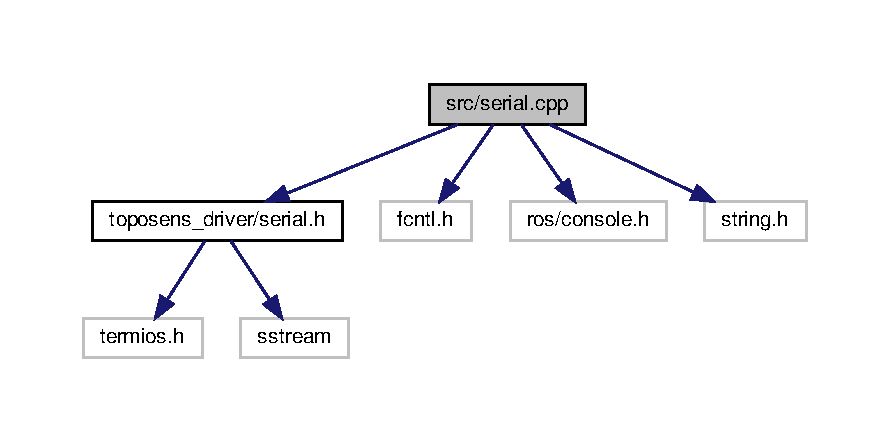
\includegraphics[width=350pt]{serial_8cpp__incl}
\end{center}
\end{figure}


\subsection{Detailed Description}
Implements serial interface to a TS sensor using native Unix command structures. 

\begin{DoxyAuthor}{Author}
Adi Singh, Sebastian Dengler 
\end{DoxyAuthor}
\begin{DoxyDate}{Date}
January 2019
\end{DoxyDate}
Uses ros/console.\+h for outputting R\+O\+S-\/style string messages to terminal. 